\graphicspath{{chapters/03/media/}}
\chapter{Processamento dei dati}
\label{cha:processamento}
Definito in \S\ref{cha:intro} l'obiettivo di questo progetto si deve definire una pipeline che, da dati di sequenziamento di RNA e da una lista di SNP esonici  sia in grado di fornire le istanze di espressione allelo-specifica.
Questa pipeline viene definita basandosi su quella presentata in \cite{ase_pipeline} e si compone pertanto di tre fasi principali:
\begin{enumerate}
	\item Pre-processamento e allineamento dei dati di RNA-seq, con eventuale deduplicazione e ricalibrazione.
	\item Analisi di dati \emph{WES} in modo da ottenere una lista di possibili SNP esonici da considerare.
	\item Calcolo dei dati di sbilanciamento allelico.
\end{enumerate}
La figura \ref{fig:proj_pipeline} \`e una visualizzazione della pipeline e dei tool utilizzati.\\
Essendo che questo lavoro prevede il processamento di un gran numero di file, unito al fatto che l'implementazione dei tool utilizzati pemette lo sfruttamento delle pipe di unix e la possibilit\`a di un esecuzione in multi-threading \`e stato di fondamentale importanza l'utility parallel \cite{parallel}.
Questo tool permette di trasformare l'output di un programma in parametri per un successivo e consente di decidere quante istanze del secondo possono essere eseguite contemporaneamente.\\
In particolare nel caso di STAR (\S\ref{subsec:star}) \`e stata notata una diminuzione lineare delle performance per thread del tool.
Parallel permette di mitigare questo problema in modo da, invece di eseguire un'unica istanza di star con moltissimi thread, di averne diverse in contemporanea con meno thread.
In questo modo aumenta il tempo di esecuzione di un'istanza di STAR, ma il tempo di esecuzione globale diminuisce.\\
Si nota pertanto che parallel permette non solo un'elegante implementazione della pipeline, ma fornisce un livello di controllo tale da sfruttare completamente la potenza computazionale disponibile, riducendo in questo modo il tempo globale di esecuzione.

  \begin{figure}[H]
    \label{fig:proj_pipeline}
    \centering
    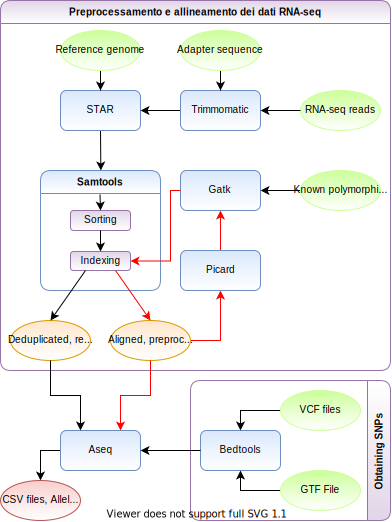
\includegraphics[scale=0.2]{pipeline.png}
    \caption{Pipeline per l'ottenimento dei dati di allelic imbalance}
  \end{figure}

  \section{Pre-processamento e allineamento dei dati RNA-seq}
  \label{sec:pre_all_rna_seq}
  Il primo passo della pipeline appena definita \`e il pre-processamento e l'allineamento dei dati RNA-seq.
  L'input della pipeline sono dei \emph{FASTQ}, file di testo che contengono i dati di sequenziamento raccolti in laboratorio. 
  Questi file subiscono un processo di preparazione in modo da ottenere dei file di allineamento utilizzabileiper ottenere i dati di sbilanciamento allelico.
  Opzionalmente i file di allineamento possono subire ulteriori modifiche prima di passare alla prossima fase in modo da tentare di migliorare i risultati ottenuti.
  Tali modifiche sono in particolare deduplicazione e ricalibrazione.

  	\subsection{Trimmomatic}
	Trimmomatic \cite{trimmomatic} \`e il primo tool ad essere utilizzato.
	Il suo obiettivo \`e quello di eliminare dalle read la sequenza adattatrice, un artificio aggiunto al RNA per rendere possibile il sequenziamento, o suoi frammenti.
	Essendo le RNA-seq fornite single-ends\footnote{Punta a spiegazione nel capitolo 1} viene utilizzata la simple mode del tool.
	Questa scansiona ogni read dalla terminazione $5'$ alla $3'$ per determinare la presenza della sequenza adattatrice.
        La scansione avviene attraverso il metodo ``seed and extend'' per trovare corrispondenze iniziali, anche non perfette, tra la read e la sequenza adattatrice.
	Successivamente svolge un allineamento locale a cui assegna uno score.
        Se lo score \`e maggiore di una soglia predefinita l'allineamento e la porzione che lo segue sono rimossi.
	Questa modalit\`a permette di identificare ogni sequenza adattatrice in ogni luogo della read a patto che l'allineamento sia abbastanza lungo e la read abbastanza accurata.
	Si nota per\`o come nelle regioni dove solo una corta corrispondenza parziale \`e possibile, come alle estremit\`a della read, i contaminanti non possono essere identificati attendibilmente.
	Oltre alla rimozione delle sequenze adattatrici Trimmomatic tronca un'estremit\`a secondo un algoritmo di filtraggio secondo qualit\`a.
	Tra i metodi forniti dallo strumento \`e stato utilizzato quello del ``sliding window quality filtering'':
	scansiona la read dal $5'$ e rimuove la terminazione $3'$ quando la qualit\`a media di un gruppo di basi scende sotto una soglia specificata.
	Il risultato di questo passaggio sar\`a un altro fastq file con le sequenze adattatrici rimosse.
        \begin{table}[H]
                \begin{tabular}{|c|c|}
                        \hline
                        Parametro & Valore\\
                        \hline
                        ILLUMINACLIP: & TruSeq3-SE.fa:2:30:10\\
                        \hline
                        phred & $33$\\
                        \hline
                        LEADING: & $3$\\
                        \hline
                        TRAILING: & $3$\\
                        \hline
                        SLIDINGWINDOW: & $4:15$\\
                        \hline
                        MINLEN: & $36$\\
                        \hline
                 \end{tabular}
                 \centering
                 \caption{Parametri utilizzati per trimmomatic}
        \end{table}

	\subsection{Star}
	\label{subsec:star}
	Star (spliced transcript alignment to a riferimento) \cite{star} \`e il secondo tool della pipeline.
	Prende come input il file fastq generato da Trimmomatic e un genoma di riferimento.
        Allinea poi i dati di sequenziamento al riferimento in modo da determinare il luogo del genoma che ha originato le read e producendo i file di allineamento.
	Questo tool \`e stato creato con l'obiettivo di allineare RNA-seq di media-grande lunghezza, a differenza dei suoi competitori che, essendo creati a partire da allineatori per dati di DNA, hanno un maggiore tasso di errore.
        Star infatti tenta di risolvere problemi di allineamento dovuti agli eventi di splicing che avvengono durante la creazione delle molecole di mRNA.
        Per farlo deve tentare di creare allineamenti accurati di read contenenti mal-accoppiamenti, inserzioni o delezioni causati da variazioni genomiche o errori di sequenziamento.
        Lo fa mappando contemporaneamente sequenze derivate da regioni genomiche non contigue unite da eventi di splicing.
        Il processo di allineamento di star avviene in due fasi.\\
	La prima fase o \emph{seed search} consiste della ricerca sequenziale di \emph{Maximal Mappable Prefix MMP}.
	Data una sequenza $R$, una regione $i$ e un genoma di riferimento $G$, $MMP(R, i, G)$ \`e la pi\`u lunga sottostringa $(R_i, R_{i+1}, \dots, R_{i+MML-1})$ che corrisponde esattamente a una o pi\`u sottostringhe di $G$.
	$MML$ \`e la massima lunghezza mappabile.
	La seed search permette quindi un'identificazione di giunzioni di splicing senza nessuna conoscenza a priori.
	L'implementazione attraverso \emph{Uncompressed suffix arrays} causa alla complessit\`a dell'algoritmo di scalare logaritmicamente con la lunghezza del genoma di riferimento.
	Gli array sono non compressi per permettere tempi di ricerca pi\`u veloci, ma causano un aumento del consumo di memoria (circa $27GB$ per il genoma umano).\\
	La seconda fase o \emph{clustering, stitching and scoring} consiste nel costruire allineamenti dell'intera sequenza di read unendo tutti i seed allineati al genoma nella prima fase.
        Viene scelto un seed ancora a cui tutti gli altri sono raggruppati insieme: tutti quelli che si trovano al di sotto di una certa distanza formano una \emph{genomic window}.
        Il seed ancora viene scelto limitando il numero di loci genomici a cui si allinea.
        Tutti i seed che sono stati mappato nella \emph{genomic window} sono successivamente uniti insieme assumendo un modello lineare locale di trascrizione.
	Il processo di unione viene guidato da un sistema di punteggi che penalizza mal-accoppiamenti, inserzioni, delezioni e \emph{splice junction gap}.
	Star ha come output un sam (sequence alignment map) file contenente le sequenze di input allineate rispetto al genoma di riferimento.
        La sezione di allineamento dell'output \`e formata da record separati da tabulazioni contenenti informazioni sulla sequenza, su dove \`e stata allineata e sulla qualit\`a dell'allineamento.
        Crea inoltre una stringa \emph{CIGAR} utile a valle della pipeline.
        \begin{table}[H]
              \centering
              \begin{tabular}{|c|c|}
                      \hline
                      Parametro & Valore\\
                      \hline
                      Genoma di riferimento & GRCh38\\
                      \hline
                      outSamstrandField & intronMotif\\
                      \hline
                      outSAMunmapped & None\\
                      \hline
                      outReadsUnmapped & fastx\\
                      \hline
                      outFilterScoreMinOverLread & $0.33$\\
                      \hline
                      outFilterMatchNminOverLread & $0.33$\\
                      \hline
              \end{tabular}
              \caption{Parametri utilizzati per star}
        \end{table}

	\subsection{Samtools}
	I samtools \cite{samtools} sono un insieme di programmi necessari per interagire con i dati di allineamento.
	Nella pipeline sono utilizzati per compiere delle operazioni sui sam file generati da star (\S\ref{subsec:star}) in modo da prepararli prima che possano essere utilizzati successivamente per generare i dati di sbilanciamento allelico (\S\ref{sec:aseq}).
        In particolare svolgono le operazioni di ordinamento, indicizzazione e compressione dei file di input.
        Questo avviene attraverso due programmi: samtools sort \cite{samtools-sort} e samtools index \cite{samtools-index}.
        Il primo ordina gli allineamenti secondo le coordinate di inizio e comprime implicitamente l'input in formato bam (binary alignment map).
        Il secondo invece crea, a partire dall'output del programma sort un indice in formato bai di tale file, permettendo efficienti operazioni di accesso casuale al bam file.
        L'output finale \`e un bam file ordinato e indicizzato che pu\`o essere utilizzato come input di aseq.

	\subsection{Deduplicazione e ricalibrazione}
        \label{subsec:deduprecab}
	La deduplicazione e la ricalibrazione sono due processi di elaborazione dei dati di RNA-seq che tentano di risolvere errori presenti nei bam file che sono stati allineati attraverso star (\S\ref{subsec:star}).
  Questi due passaggi vengono svolti attraverso una serie di tools eseguiti sequenzialmente come si nota nella figura \ref{fig:pipeline_deduprecal}.
  \begin{figure}[H]
    \label{fig:pipeline_deduprecal}
    \centering
    \includegraphics[scale=0.17]{deduprecal.png}
    \caption{Pipeline di deduplicazione e ricalibrazione}
  \end{figure}
  Il primo passaggio viene svolto dal tool \emph{AddOrReplaceReadGroups} \cite{addorreplacegroup} di Picard \cite{picard}, un passaggio di preparazione delle read necessario a tutti i tool successivi.
  Questo assegna tutte le read in un file a un nuovo read-group settando un campo nel BAM file, in modo da assegnare tutte le read a un genotipo specifico.
  \begin{table}[H]
        \centering
        \begin{tabular}{|c|c|}
                \hline
                Parametro & Valore\\
                \hline
                RGID & $1$\\
                \hline
                RGLB & lib1\\
                \hline
                RGPL & ILLUMINA\\
                \hline
                RGPU & unit1\\
                \hline
                RGSM & $20$\\
                \hline
         \end{tabular}
         \caption{Parametri utilizzati per AddOrReplaceReadGroups}
    \end{table}

    \subsubsection{Deduplicazione}
    Il processo di deduplicazione e le motivazioni dietro alla sua utilit\`a sono definite in \cite{dedup}
    Si definiscono come read duplicate in un BAM file delle read che si generano da un singolo frammento di RNA.
    Possono originarsi durante la preparazione del campione, per esempio durante la costruzione della libreria attraverso PCR o risultare da un singolo cluster di amplificazione, identificato incorrettamente come cluster multipli dal sensore ottico dello strumento di sequenziamento.\\
    Il processo di deduplicazione \`e stato svolto attraverso il tool \emph{MarkDuplicates} di Picard.
    Il programma compara le sequenze nelle posizioni $5'$ sia delle read che dei read-pairs.
    Dopo che ha trovato tutti le read duplicata queste vengono ordinate secondo la somma dei punteggi di qualit\`a delle basi.
    La read con il punteggio pi\`u alto viene considerata primaria, le altre duplicati.
    Grazie all'opzione \emph{REMOVE\_DUPLICATE=true} tutte le sequenze duplicate vengono rimosse.
    Viene infine ricreato l'indice del BAM file attraverso \emph{samtools index}.
    \begin{table}[H]
        \centering
        \begin{tabular}{|c|c|}
                \hline
                Parametro & Valore\\
                \hline
                REMOVE\_DUPLICATES & true\\
                \hline
                MAX\_FILE\_HANDLES\_FOR\_READ\_ENDS\_MAP & $1000$\\
                \hline
                VALIDATION\_STRINGENCY & LENIENT\\
                \hline
                ASSUME\_SORTED & true\\
                \hline
         \end{tabular}
         \caption{Parametri utilizzati per MarkDuplicates}
    \end{table}

    \subsubsection{Ricalibrazione}
    La ricalibrazione viene svolta da una serie di tool facenti parte della suite Gatk \cite{gatk}.
    Il processo si compone di due fasi:
    \begin{multicols}{2}
      \begin{enumerate}
        \item Riallineamento degli indels definito in \cite{indelrealign}.
        \item Ricalibrazione delle basi basata sul punteggio di qualtit\`a definito in \cite{bqsr}.
      \end{enumerate}
    \end{multicols}
    Il primo passaggio, svolto dal tool \emph{SplitNCigarReads} \cite{splitncigarreads}, progettato specificatamente per dati di RNA-seq, \`e necessario per il corretto funzionamento degli step successivi.
    In un file BAM di RNA-seq infatti si trovano stringhe \emph{CIGAR} che descrivono come una base in ogni read \`e mappata.
    Il valore $N$ corrisponde a una base saltata sul genoma di riferimento.
    Nel caso di RNA-seq tali basi possono corrispondere o a sequence introniche, non presenti nel RNA a causa dello splicing o a sequenze di ``overhang'' che potrebbero portare a falsi positivi.
    \emph{SplitNCigarReads} elimina le basi corrispondenti a una $N$ da una read separandola in due: una che finisce a destra e l'altra che inizia a sinistra della base rimossa.
    Il risultato di questo processo \`e la separazione degli esoni in read diverse e un'eliminazione degli overhang.
    Come risultato gli esoni del RNA vengono separati in segmenti e gli overhang eliminati in modo da non causare falsi positivi.\\
    Dopo questo lavoro di processamento inizia la fase di riallineamento degli indels.
    \begin{table}[H]
        \centering
        \begin{tabular}{|c|c|}
                \hline
                Parametro & Valore\\
                \hline
                R & Homo\_Sapiens.GRCh38.dna.primary\_assembly.fa\\
                \hline
                U & ALLOW\_N\_CIGAR\_READS\\
                \hline
         \end{tabular}
         \caption{Parametri utilizzati per SplitNCigarReads}
    \end{table}
    
    \paragraph{Riallineamento locale degl indel}
    Il riallineamento locale degli indels \`e necessario in quanto permette di correggere errori sistematici causati dall'allineatore genomico.
    Una limitazione di questi allineatori infatti \`e che considerano ogni read in maniera indipendente: le strategie di assegnazione dei punteggi limitano la loro abilit\`a di allineare accuratamente in presenza di indel.
    Il processo di allineamento locale considera invece tutte le read che attraversano una posizione in modo da ottenere un consenso di alto punteggio che supporta la presenza di un evento di indel.
    Il riallineamento viene svolto attraverso l'utilizzo di due tool: \emph{RealignerTargetCreator} e \emph{IndelRealigner}.
    Il primo prende come input un BAM file ordinato e indicizzato e a partire da esso genera un file di output formato da una lista a una colonna contenente gli intervalli.
    Ogni reecord di questo file degli intervalli rappresenta un potenziale sito dove \`e avvenuto un indel.
    Infine se gli intervalli sono prossimali vengono uniti in un intervallo unico.
    Il secondo tool prende come input lo stesso BAM di \emph{RealignerTargetCreator} e il file di intervalli da esso generato e svolge un riallineamento locale sulle read coincidenti con l'intervallo target usando consensi dagli indel presenti nell'allineamento originale.
    L'output \`e un BAM ordinato e indicizzato.
    \begin{table}[H]
        \centering
        \begin{tabular}{|c|c|}
                \hline
                Parametro & Valore\\
                \hline
                S & SILENT\\
                \hline
                R & Homo\_Sapiens.GRCh38.dna.primary\_assembly.fa\\
                \hline
                nt & $10$\\
                \hline
         \end{tabular}
         \caption{Parametri utilizzati per RealignerTargetCreator}
    \end{table}
                
    \begin{table}[H]
        \centering
        \begin{tabular}{|c|c|}
                \hline
                Parametro & Valore\\
                \hline
                targetIntervals & file prodotto da RealignerTargetCreator\\
                \hline
                R & Homo\_Sapiens.GRCh38.dna.primary\_assembly.fa\\
                \hline
         \end{tabular}
         \caption{Parametri utilizzati per IndelRealigner}
    \end{table}
    
    \paragraph{Ricalibazione delle basi basata sul punteggio di qualit\`a}
    Il processo di ricalibrazione delle basi basato sul punteggio di qualit\`a serve a risolvere errori generati durante il sequenziamento.
    Si definisce il punteggio di qualit\`a di una base come una stima dell'errore emesso dalla macchina di sequenziamento: esprimono quanto questa \`e confidente che ha chiamato la base corretta ogni volta.
    Questi punteggi sono soggetti a varie sorgenti di errori tecnici dovuti alla fisica o alla chimica di come una reazione di sequenziamento funziona o a difetti nell'equipaggiamento.
    Gli errori portano pertanto a una sottostima o sovrastima (tipicamente la seconda) del punteggio di qualit\`a fornito dal macchinario di sequenziamento.
    Per tentare di risolvere si utilizza machine learning per modellarli empiricamente a modificare i valori di qualit\`a migliorarne la veridicit\`a.
    La ricalibrazione delle basi avviene attraverso l'utilizzo di due tool.
    Il primo \`e \emph{BaseRecalibrator} \cite{baserecalibrator} e costruisce un modello di covarianza da un BAM e da un insieme di varianti conosciute in un file VCF e lo salva in un file.
    Le varianti conosciute sono usate per mascherare basi ai siti di variazioni aspettate in modo da non considerarle come errori.
    Al di fuori di queste eccezioni ogni mal-accoppiamento viene contato come un errore.
    Per costruire il modello di ricalibrazione il tool tabula i dati del BAM secondo il read group, il punteggio di qualit\`a, il ciclo della macchina che ha prodotto la base, la base corrente e successiva.
    Successivamente si conta il numero di basi e quanto spesso queste hanno un mal-accoppiamento con la base di riferimento.
    Il secondo tool \emph{PrintReads} \cite{printreads} applica il modello creato dal primo al BAM di input, aggiornandolo cos\`i ai punteggi di qualit\`a migliorati.
    Infine viene ricreato l'indice del BAM file attraverso \emph{samtools index}.\\
    In questo modo si \`e creato un file BAM pronto per essere utilizzato da ASEQ.
    \begin{table}[H]
        \centering
        \begin{tabular}{|c|c|}
                \hline
                Parametro & Valore\\
                \hline
                knownSites & lista di VCF contenente gli SNP conosciuti\\
                \hline
                R & Homo\_Sapiens.GRCh38.dna.primary\_assembly.fa\\
                \hline
                nct & $10$\\
                \hline
         \end{tabular}
         \caption{Parametri utilizzati per BaseRecalibrator}
    \end{table}
                
    \begin{table}[H]
        \centering
        \begin{tabular}{|c|c|}
                \hline
                Parametro & Valore\\
                \hline
                nct & $10$\\
                \hline
                R & Homo\_Sapiens.GRCh38.dna.primary\_assembly.fa\\
                \hline
                BQSR & Modello output di BaseRecalibrator\\
                \hline
         \end{tabular}
         \caption{Parametri utilizzati per PrintReads}
    \end{table}
    

  \section{Ottenimento degli SNP di interesse}
  Una volta ottenuti i file di allineamento si rende necessario ottenere una lista di SNP dei quali si vuole ottenere il valore di sbilanciamento allelico.
  Per ottenere questi dati sono stati utilizzati il file GTF\footnote{Sezione dati input} contenente informazioni sulla porzione esonica del genoma umano e da un insieme di VCF divisi per cromosoma contenenti le informazioni riguardo le varianti ottenute negli essere umani.
  Dopo aver ristretto i VCF agli SNP sono stati intersecati con il file GTF.
  L'intersezione \`e stata volta dal tool \emph{bedtools intersect} \cite{bedtoolsintersect}, facente parte della suite bedtools \cite{bedtools}.
  Questo tool ha permesso di trovare ogni record del VCF presente anche nel GTF.
  In questo modo \`e stato creato un insieme di file VCF, uno per ogni cromosoma, contiene ogni SNP presente nella parte esonica del genoma.
  La restrizione alla parte esonica del genoma non causa alcuna perdita di potere predittivo in quanto si stanno considerando dati di RNA-seq, ma permette una significativa diminuzione del carico computazionale svolto da aseq (\S\ref{sec:aseq}).
  I VCF risultanti da questo processo sono pronti per essere utilizzati come input di aseq.
  \begin{table}[H]
        \centering
        \begin{tabular}{|c|c|}
                \hline
                Parametro & Valore\\
                \hline
                wa & non richiesto\\
                \hline
                u & non richiesto\\
                \hline
                a & VCF file\\
                \hline
                b & GTF file\\
                \hline
         \end{tabular}
         \caption{Parametri utilizzati per bedtools intersect}
  \end{table}

  \section{Calcolo dei dati di sbilanciamento allelico}
  \label{sec:aseq}
  Per computare i valori di sbilanciamento allelico \`e stato utilizzato aseq \cite{aseq}.
  Questo tool tenta di risolvere alcune limitazioni di altri programmi di analisi di espressione allelo-specifica.
  Non richiede infatti informazioni genomiche dei genitori dell'individuo e non si basa unicamente sui dati di RNA-seq.
  Aseq in particolare accoppia dati di sequenziamento di nuova generazione trascrittomici e genomici in modo da superare queste limitazioni.
  La sua implementazione sfrutta le API di samtools, permettendo rapide funzionalit\`a di accesso casuale su file di allineamento inidicizzate e ne aumenta il potere computazionale attraverso il multi-threading.
  Delle modalit\`a che aseq fornisce \`e stata utilizzata quella principale di analisi ASE, ponendo limitazioni solo sulla qualit\`a delle basi e la qualit\`a delle letture dei file di allineamento.
  In questo modo aseq non restringe l'output agli eventi di ASE che individua ma ritorna il valore del pileup per ogni SNP datogli in input.
  Il pileup \`e un formato che riassume le chiamate delle basi rispetto a una sequenza di riferimento.
  Pertanto aseq computa per ogni SNP nella lista, a partire dal nome, dalla base canonica e dalla base alternativa, il coverage per tale SNP, la qualit\`a della chiamata della base e la frazione allelica.
  Questo permette di applicare all'output diversi filtri successivamente durante l'analisi cosicch\`e da poter trovare i valori soglia ottimali per ottenere risultati significativi in un secondo momento senza ripetere continuamente la computazione del pileup e snellendo il carico computazionale dell'analisi.
  Non si sfrutta pertanto il potere di individuazione di eventi di ASE da parte di aseq, ma solo il suo veloce engine computazionale che permette di aumentare l'efficienza della creazione dei dati di pileup per una singola base.
  Ora, dopo aver prodotto i file di allineamento dai dati di RNA-seq dei campioni e la lista di SNP esonici di interesse si pu\`o procedere all'esecuzione di aseq.
  In particolare i file di allineamento sono divisi in due insiemi: uno creato dopo l'allineamento con star (\S\ref{subsec:star}) e l'altro dopo il processo di deduplicazione e ricalibrazione (\S\ref{subsec:deduprecab}).
  Ognuno di questi insiemi possiede un file per campione\footnote{Riferimento a lista di campioni}.
  La lista di SNP si trova invece in un insieme di file VCF, un file per ogni autosoma, uno per il cromosoma $X$ e uno per il DNA mitocondriale.
  Perci\`o per ogni file di allineamento viene eseguito aseq per ogni file VCF, ottenendo in questo modo i dati di pileup di ogni SNP per ogni campione divisi per cromosoma.
  L'output di aseq \`e un file di testo delimitato da tabulazioni, formato che rende facilmente ottimizzabili le successive analisi attraverso tool come awk, sed o framework come pandas per python o tidyverse per R.
  \begin{table}[H]
        \begin{tabular}{|c|c|}
                \hline
                Parametro & Valore\\
                \hline
                bam & BAM file indicizzato prodotto precedentemente\\
                \hline
                vcf & VCF file ottenuto precedentemente\\
                \hline
                mbq & $20$\\
                \hline
                mrq & $20$\\
                \hline
         \end{tabular}
         \centering
         \caption{Parametri utilizzati per aseq}
   \end{table}
  
